\documentclass[11pt]{article}

\usepackage[margin=1in]{geometry}
\usepackage{amsmath,amssymb,amsthm}
\usepackage{booktabs}
\usepackage{enumitem}
\usepackage{graphicx}
\usepackage{hyperref}
\usepackage{placeins}
\usepackage{xcolor}

\hypersetup{
  colorlinks=true,
  linkcolor=blue,
  citecolor=blue,
  urlcolor=blue
}

\newtheorem{definition}{Definition}
\newtheorem{proposition}{Proposition}
\newtheorem{remark}{Remark}

\newcommand{\R}{\mathbb{R}}
\newcommand{\Cov}{\operatorname{Cov}}
\newcommand{\spanop}{\operatorname{span}}

\title{A Compact Narrative for Prediction-Relevant Operator Mechanisms}
\author{Fernando Ruiz Mazo}
\date{May 1, 2026}

\begin{document}

\maketitle

\section{The Question}

The starting point is a simple ambiguity. A transformer trained for in-context linear regression may
make predictions close to linear-kernel ridge regression, but pointwise accuracy on one sampled
label vector does not identify the computation being used. Many algorithms can agree with ridge
regression on the realized labels while responding differently to nearby counterfactual labels.

The note therefore changes the object of study. Instead of asking only whether the transformer
predicts the right targets for one sampled context, it freezes the input geometry and perturbs only
the context labels. The first question becomes:
\[
\text{When labels are changed infinitesimally, does the transformer respond like the ridge operator?}
\]
This operator-response test is only the entry point. The paper then asks a stronger mechanistic
question: if the transformer has a ridge-like local response, when does a hidden layer contain a
compact context-side subspace sufficient to reconstruct the ridge operator at the prediction-risk
scale of the task?  Causal use is then a separate intervention question: after a sufficient subspace
has been identified, do interventions preserving or removing that subspace preserve or damage the
transformer's response?

The resulting claim is stronger than behavioral imitation but narrower than global equality. In the
successful regimes, the transformer locally realizes the task-distributed ridge label-response
operator, and hidden response spans contain low-dimensional subspaces whose induced reduced KRR
operators recover exact KRR up to a predeclared prediction-risk tolerance. The number of required
directions is computed before looking at activations. The locality matters: the tests concern the
sampled geometry, the chosen perturbation scale, and especially task-label directions rather than
all possible label perturbations.

\section{Fixed Geometry Makes Ridge Regression an Operator}

Fix one in-context episode with context and target inputs
\[
X_{\mathrm{ctx}}\in\R^{n_{\mathrm{ctx}}\times d_x},
\qquad
X_{\mathrm{tgt}}\in\R^{n_{\mathrm{tgt}}\times d_x}.
\]
The fixed geometry is
\[
G=(X_{\mathrm{ctx}},X_{\mathrm{tgt}}).
\]
During the operator tests, \(G\) is held fixed. The context inputs do not move, the target inputs do
not move, and the only varying object is the context-label vector
\[
y=(y_1,\ldots,y_{n_{\mathrm{ctx}}})\in\R^{n_{\mathrm{ctx}}}.
\]
Define
\[
K=X_{\mathrm{ctx}}X_{\mathrm{ctx}}^\top,\qquad
K_t=X_{\mathrm{tgt}}X_{\mathrm{ctx}}^\top,\qquad
A=K+\sigma^2 I.
\]
For linear-kernel ridge regression, the dual coefficients and target predictions are
\[
\alpha^\star=A^{-1}y,\qquad
y^\star=K_t\alpha^\star=K_tA^{-1}y.
\]
Thus, once \(G\) is fixed, ridge regression is a linear map from context labels to target
predictions:
\[
T_G:=K_tA^{-1},
\qquad
T_G:\R^{n_{\mathrm{ctx}}}\to\R^{n_{\mathrm{tgt}}}.
\]

The transformer defines a map on the same spaces:
\[
F_\theta^G:\R^{n_{\mathrm{ctx}}}\to\R^{n_{\mathrm{tgt}}},
\qquad
F_\theta^G(y)=\widehat y_\theta.
\]
When the geometry is clear, write \(T\) and \(F\). The central comparison is not merely
\(F(y)\approx Ty\) for one \(y\). It is whether the local response of \(F\) to label perturbations
matches the operator \(T\).

\section{Context-Label Directions, Local Operators, and Additivity}

A context-label direction is a vector
\[
u\in\R^{n_{\mathrm{ctx}}}.
\]
It assigns one scalar to each context example. Perturbing in direction \(u\) means changing labels as
\[
y+\varepsilon u
=
(y_1+\varepsilon u_1,\ldots,y_{n_{\mathrm{ctx}}}+\varepsilon u_{n_{\mathrm{ctx}}}).
\]
This is a direction over context positions. It is not a direction in input-feature space and not a
direction in target space. If there are 47 context examples, these directions live in \(\R^{47}\).

Pointwise agreement checks only the value of two maps at one label vector:
\[
F(y)\approx Ty.
\]
Since fixed-geometry ridge regression is linear, its Jacobian is the operator itself:
\[
J_T(y)=T\quad\text{for every }y.
\]
The transformer map \(F\) can be nonlinear in the labels. The weakest local version of ``the same
label-to-prediction rule'' is therefore equality of first-order responses:
\[
J_F(y)u\approx Tu.
\]
Equivalently, for small label perturbations,
\[
F(y+\delta)\approx F(y)+T\delta.
\]
The experiments estimate the Jacobian action with the central finite difference
\[
D_\varepsilon F(y)[u]
:=
\frac{F(y+\varepsilon u)-F(y-\varepsilon u)}{2\varepsilon}.
\]
The symmetric form is used because it cancels the leading first-order bias of a one-sided
difference: for a smooth map, the error is \(O(\varepsilon^2)\) rather than \(O(\varepsilon)\). It also
treats positive and negative label perturbations in the same direction symmetrically, which is
important when the goal is to estimate the local tangent response rather than a one-sided effect.
The behavioral operator test asks whether
\[
D_\varepsilon F(y)[u]\approx Tu
\]
on held-out label directions.

This is still a local statement. Matching the value and first derivative at one point does not imply
global equality. For example, \(f(x)=x+x^2\) and \(g(x)=x\) have the same value and derivative at
\(x=0\), but differ away from zero. Thus derivative matching supports tangent-level agreement,
not \(F(y')=Ty'\) for all possible labels.

The probe distribution specifies which counterfactual label directions are tested. The main probes
are task-label probes:
\[
u\sim\mathcal{N}(0,A).
\]
This is the natural law because, under the matched linear task
\[
y=X_{\mathrm{ctx}}\beta+\eta,\qquad
\beta\sim\mathcal{N}(0,I),\qquad
\eta\sim\mathcal{N}(0,\sigma^2I),
\]
conditioning on the fixed geometry leaves only \(\beta\) and \(\eta\) random, so
\[
y\mid G\sim\mathcal{N}(0,X_{\mathrm{ctx}}X_{\mathrm{ctx}}^\top+\sigma^2I)
=\mathcal{N}(0,A).
\]
Equivalently, the conditional label covariance is
\[
\Cov(y\mid G)=A.
\]
Thus \(u\sim\mathcal{N}(0,A)\) samples counterfactual label perturbations with the same covariance
geometry as labels generated by the task, after the input geometry has been fixed. In this precise
sense, task probes are the directions the task distribution itself emphasizes. In whitened coordinates,
they are \(u=A^{1/2}z\), \(z\sim\mathcal{N}(0,I)\). The experiments also use isotropic probes
\[
u\sim\mathcal{N}(0,I),
\]
which test arbitrary context-label directions equally. The distinction is central: the claim is
task-local because the transformer is close to ridge on task-label probes but not on arbitrary
isotropic probes. Build probes are used to construct subspaces or fitted controls; held-out probes
are used for reported errors.

For a held-out probe set \(U=\{u_1,\ldots,u_m\}\) and a fixed linear operator
\(S:\R^{n_{\mathrm{ctx}}}\to\R^{n_{\mathrm{tgt}}}\), define
\[
E_\varepsilon(F,S;U)
:=
\left(
\frac{
\sum_{j=1}^m\|D_\varepsilon F(y)[u_j]-Su_j\|_2^2
}{
\sum_{j=1}^m\|Tu_j\|_2^2+\eta_{\mathrm{num}}
}
\right)^{1/2}.
\]
When \(S=T\), this measures whether the transformer's finite-difference response matches exact
ridge regression. The denominator normalizes by the ridge-response energy on the same probes, so
an error of \(0.01\) means a root-mean-square discrepancy of about one percent of the typical ridge
response size.

\begin{proposition}[Transformer errors are not bounded by 1]
For a finite probe set \(U\), write
\[
R_U^2=\sum_j\|Tu_j\|_2^2.
\]
If \(D_\varepsilon F(y)[u_j]=0\) for all probes, then
\[
E_\varepsilon(F,T;U)=\frac{R_U}{(R_U^2+\eta_{\mathrm{num}})^{1/2}}\le 1.
\]
If \(D_\varepsilon F(y)[u_j]=-Tu_j\), then the same calculation gives a value at most 2. More
generally, if \(D_\varepsilon F(y)[u_j]=cTu_j\), then
\[
E_\varepsilon(F,T;U)
=
|c-1|\frac{R_U}{(R_U^2+\eta_{\mathrm{num}})^{1/2}},
\]
so transformer-response errors have no universal upper bound.
\end{proposition}

\begin{proof}
Substitute the three proposed finite-difference responses into the definition of
\(E_\varepsilon(F,T;U)\). The last expression diverges as \(|c|\to\infty\) whenever the ridge
response energy \(R_U^2\) is nonzero.
\end{proof}

Because ridge is linear, its higher-order derivatives are zero. We do not try to estimate all
higher-order derivatives of the transformer. Instead, we check whether nonlinear interactions are
small at the tested perturbation scale. Ridge has
\[
T(u+v)=Tu+Tv.
\]
A nonlinear transformer need not satisfy
\[
D_\varepsilon F(y)[u+v]\approx D_\varepsilon F(y)[u]+D_\varepsilon F(y)[v].
\]
If this approximate additivity failed badly, then \(E_\varepsilon(F,T)\) would mix two effects:
failure to be ridge and failure to have a stable local linear response.

For paired directions \(V=\{(u_j,v_j)\}_{j=1}^m\), define the second mixed finite difference
\[
C_j =
F(y+\varepsilon u_j+\varepsilon v_j)
-F(y+\varepsilon u_j-\varepsilon v_j)
-F(y-\varepsilon u_j+\varepsilon v_j)
+F(y-\varepsilon u_j-\varepsilon v_j),
\]
and the additivity defect
\[
A_\varepsilon(F;V)
:=
\left(
\frac{
\sum_{j=1}^m\|C_j\|_2^2
}{
\sum_{j=1}^m\|T(\varepsilon u_j+\varepsilon v_j)\|_2^2+\eta_{\mathrm{num}}
}
\right)^{1/2}.
\]
For any affine function of the labels, \(C_j=0\) exactly. Because the defect is normalized by
ridge-response energy, values below one mean the non-additive interaction is smaller than the
typical ridge response on the tested paired probes; values around one mean it is ridge-scale; values
above one mean the interaction is larger than the ridge response, so a local-linear interpretation is
unreliable. This diagnostic does not identify the operator. It only says whether a local operator
comparison is meaningful at the chosen \(\varepsilon\) and probe law.

\section{Activation Subspaces and Prediction-Risk Rank}

The previous section gives behavioral certificates:
\[
F(y)\approx Ty,\qquad D_\varepsilon F(y)[u]\approx Tu.
\]
These are necessary, but they are still input-output facts. They do not say whether the transformer
represents the directions needed for ridge regression, or whether those directions are used. The
mechanistic question is: does the residual stream expose a compact set of context-position
directions sufficient for the prediction-relevant ridge computation?

This is the right internal object to look for because ridge uses context-position dual variables.
For fixed geometry,
\[
\alpha^\star(y)=A^{-1}y\in\R^{n_{\mathrm{ctx}}},
\qquad
Ty=K_t\alpha^\star(y).
\]
The dual coordinate \(\alpha_i\) is indexed by the \(i\)-th context example. The context residual
stream has the same context axis. At layer \(\ell\),
\[
H_\ell^{\mathrm{ctx}}\in\R^{n_{\mathrm{ctx}}\times D},
\]
where \(D\) is the residual width. Rows are context tokens, and the \(k\)-th column
\(H_\ell^{\mathrm{ctx}}[:,k]\) is a scalar pattern over context positions, hence a vector in
\(\R^{n_{\mathrm{ctx}}}\). Linear combinations of residual-stream columns therefore define
candidate directions in the same space as ridge dual variables.

Let
\[
Q=[q_1,\ldots,q_r]\in\R^{n_{\mathrm{ctx}}\times r}
\]
be a basis matrix for such candidate context-position directions. The subspace is the column span
\[
\spanop(Q)=\{Qc:c\in\R^r\}\subseteq\R^{n_{\mathrm{ctx}}},
\]
so \(Q\) is both a matrix representation and, by abuse of language, the subspace it spans. We use
an \(A\)-orthonormal basis,
\[
Q^\top A Q=I,
\]
because the quadratic part of the ridge dual objective is \(\frac12\alpha^\top A\alpha\). Thus the
natural size of a dual displacement is \(\alpha^\top A\alpha\), and two directions are orthogonal in
the ridge geometry when their cross-term in this quadratic energy vanishes.

Now define what it means for \(\spanop(Q)\) to be useful for ridge. This is a restriction of the
dual solution, not an ordinary restriction of the input label vector. Full ridge solves
\[
\alpha^\star(y)
=
\arg\min_{\alpha\in\R^{n_{\mathrm{ctx}}}}
\left\{
\frac12\alpha^\top A\alpha-\alpha^\top y
\right\},
\]
whose first-order condition is \(A\alpha-y=0\), hence \(\alpha^\star=A^{-1}y\). To restrict the
dual solution to \(\spanop(Q)\), write \(\alpha=Qc\). Plugging this into the same dual objective gives
\[
\frac12 c^\top Q^\top A Qc-c^\top Q^\top y.
\]
Since \(Q^\top A Q=I\), this is
\[
\frac12 c^\top c-c^\top Q^\top y.
\]
Differentiating with respect to \(c\) gives \(c-Q^\top y=0\), so
\[
c^\star=Q^\top y.
\]
Therefore the restricted dual solution is
\[
\alpha_Q(y)=QQ^\top y.
\]
Without the \(A\)-orthonormal convention, the same calculation would give
\[
\alpha_Q(y)=Q(Q^\top A Q)^{-1}Q^\top y.
\]
Predictions are still read out through the context-target kernel matrix \(K_t\), so the reduced
ridge operator induced by \(Q\) is
\[
T_Q:=K_tQQ^\top.
\]
This is the bridge from residual-stream directions to an operator-level certificate. We are not
fitting an arbitrary probe. We are asking whether the directions exposed by the residual stream are
enough so that ridge, restricted to those directions, still predicts like full ridge.

The reason this sufficiency test is prediction-relevance weighted rather than global is that not
every label direction matters equally for prediction. Conditional on the fixed geometry,
\[
y\mid G\sim\mathcal{N}(0,A).
\]
So the task naturally emphasizes perturbations
\[
u\sim\mathcal{N}(0,A),
\]
not arbitrary Euclidean directions. A direction is task-relevant when it is likely under this
covariance geometry and when ridge produces a non-negligible target response along it. This leads
to a purely ridge-theoretic benchmark: before looking inside the transformer, ask how many
directions are needed by the best possible reduced ridge response on task-distributed labels.

To turn this into a prediction-scale benchmark, we need a reference risk. The target quantity is not
the noisy context-label vector \(y\). It is the vector of latent, noise-free function values at the
target inputs. Write
\[
f_{\mathrm{tgt}}
=
\bigl(f(x^{\mathrm{tgt}}_1),\ldots,f(x^{\mathrm{tgt}}_{n_{\mathrm{tgt}}})\bigr)
\in\R^{n_{\mathrm{tgt}}},
\]
and let \(K_{tt}\) be the target-target kernel matrix. In the linear case,
\(K_{tt}=X_{\mathrm{tgt}}X_{\mathrm{tgt}}^\top\). Under the matched GP/KRR model,
\[
\begin{bmatrix}
y\\
f_{\mathrm{tgt}}
\end{bmatrix}
\Bigm|G
\sim
\mathcal{N}\!\left(
0,
\begin{bmatrix}
A & K_t^\top\\
K_t & K_{tt}
\end{bmatrix}
\right),
\]
because \(y=f_{\mathrm{ctx}}+\eta\) includes label noise while \(f_{\mathrm{tgt}}\) is the
noise-free target function. Conditioning this Gaussian gives
\[
\mathbb{E}[f_{\mathrm{tgt}}\mid y,G]=K_tA^{-1}y=Ty
\]
and
\[
\operatorname{Cov}(f_{\mathrm{tgt}}\mid y,G)
=
K_{tt}-K_tA^{-1}K_t^\top .
\]
Thus exact KRR is the posterior mean predictor of the latent target values. It still has nonzero
risk, because the noisy context labels do not determine the target function values exactly. Define
this irreducible KRR posterior prediction risk by
\[
R_{\mathrm{KRR}}(G)
:=
\mathbb{E}\|f_{\mathrm{tgt}}-Ty\|_2^2
=
\operatorname{tr}\!\left(K_{tt}-K_tA^{-1}K_t^\top\right),
\]
where the expectation is conditional on the fixed geometry \(G\).

Now compare exact KRR with any linear approximation \(S\) to \(T\). Decompose
\[
f_{\mathrm{tgt}}-Sy
=
\bigl(f_{\mathrm{tgt}}-Ty\bigr)
+
\bigl(T-S\bigr)y.
\]
The first term is the posterior residual after exact KRR, and the second term is a function of the
observed labels \(y\). Since \(Ty=\mathbb{E}[f_{\mathrm{tgt}}\mid y,G]\), the posterior residual is
orthogonal to every function of \(y\). Therefore the cross-term vanishes and
\[
\mathbb{E}\|f_{\mathrm{tgt}}-Sy\|_2^2
=
R_{\mathrm{KRR}}(G)
+
\mathbb{E}_{y\sim\mathcal{N}(0,A)}\|(T-S)y\|_2^2.
\]
The second term is the extra prediction risk caused by using \(S\) instead of exact KRR. Thus the
natural scale for deciding whether a reduced operator is good enough is not zero operator error, but
excess error relative to the irreducible risk already incurred by exact KRR. Define
\[
\rho_G(S)
:=
\frac{
\mathbb{E}_{y\sim\mathcal{N}(0,A)}\|(T-S)y\|_2^2
}{
R_{\mathrm{KRR}}(G)+\eta_{\mathrm{num}}
}.
\]
This asks how much prediction risk is added by using \(S\) instead of exact KRR.

The next question is how many source directions are needed in principle. This should be answered
before looking at the transformer. We therefore ask a purely KRR question: among all rank-\(r\)
linear responses to task-distributed labels, how much extra prediction risk is unavoidable if we
keep only \(r\) directions?

Whiten the task-label perturbations:
\[
u=A^{1/2}z,\qquad z\sim\mathcal{N}(0,I).
\]
Here \(z\) is an isotropic coordinate system for labels drawn from the task covariance \(A\). In
these coordinates, the exact KRR response is
\[
Tu=K_tA^{-1}A^{1/2}z=K_tA^{-1/2}z.
\]
Define
\[
C_G:=K_tA^{-1/2}.
\]
Thus \(C_G\) is not a new predictor. It is the same KRR operator written in coordinates where the
task-label distribution is spherical. This distinction matters. Singular values of \(T\) measure
response size to raw Euclidean label directions \(u\sim\mathcal{N}(0,I)\), which is not the task
law. Singular values of \(C_G\) measure response size to label directions that the task actually
generates, \(u\sim\mathcal{N}(0,A)\).

Let
\[
C_G=U\operatorname{diag}(s_i)V^\top,
\qquad
s_1\ge s_2\ge\cdots\ge0.
\]
If \(z\) points along the right singular vector \(v_i\), the KRR prediction moves in the
corresponding target direction with size \(s_i\). Thus \(s_i^2\) is the squared prediction-response
energy carried by the \(i\)-th task-label mode. Since \(z\) is isotropic,
\[
\mathbb{E}\|C_Gz\|_2^2=\sum_i s_i^2.
\]
Now suppose we approximate exact KRR by a rank-\(r\) linear operator. In whitened coordinates this
means approximating \(C_G\) by a rank-\(r\) matrix. By Eckart--Young, the best possible rank-\(r\)
approximation keeps the \(r\) largest singular directions. The unavoidable task-law mean squared
operator error is the discarded tail
\[
\sum_{i>r}s_i^2.
\]
Equivalently, the best possible rank-\(r\) predictor has total prediction risk
\[
R_{\mathrm{KRR}}(G)+\sum_{i>r}s_i^2.
\]
This is why the tail is compared to \(R_{\mathrm{KRR}}(G)\), not to zero and not only to the total
response energy \(\sum_i s_i^2\). The practical question is whether throwing away the tail changes
prediction performance by an amount that is negligible relative to the uncertainty already left by
exact KRR.

\begin{definition}[Prediction-risk rank]
For fixed geometry \(G\) and tolerance \(\alpha>0\), define
\[
r_\alpha(G)
:=
\min\left\{
r:
\sum_{i>r}s_i^2
\le
\alpha R_{\mathrm{KRR}}(G)
\right\}.
\]
\end{definition}

In the experiments below we write \(r_T:=r_{5\%}\), i.e. \(\alpha=0.05\). This means that \(r_T\) is
the smallest rank for which an optimally chosen reduced KRR response would have prediction risk at
most
\[
(1.05)\,R_{\mathrm{KRR}}(G).
\]
Thus \(r_T\) is not the algebraic rank of \(T\), and it is not the number of nonzero singular values.
It is the number of task-relevant KRR directions needed to be prediction-equivalent to exact KRR at
the declared tolerance. Directions beyond \(r_T\) may be mathematically nonzero, but their combined
effect on target prediction is below the chosen risk budget.

This is a finite-episode benchmark. It is computed from the sampled KRR operator before looking at
activations. If \(\dim\spanop(Q)<r_T\), then no rank-\(\dim\spanop(Q)\) reduced KRR operator can
reach the five-percent prediction-risk tolerance. If \(\dim\spanop(Q)\ge r_T\), success is still not
automatic: the span must align with the leading right singular directions of \(C_G\), because those
are the task-label modes that exact KRR uses for prediction.

The same definition applies to nonlinear kernels after replacing \(K\) and \(K_t\) by the
corresponding finite kernel matrices. No population spectral assumption is needed for the
experiments below.

\begin{proposition}[Prediction-risk excess for \(T_Q\)]
Let \(u=A^{1/2}z\), \(z\sim\mathcal{N}(0,I)\), and let \(Q^\top A Q=I\). With
\[
C=K_tA^{-1/2},\qquad W=A^{1/2}Q,\qquad P_Q=WW^\top,
\]
the reduced-operator excess risk satisfies
\[
\rho_G(T_Q)
=
\frac{\|C(I-P_Q)\|_F^2}{R_{\mathrm{KRR}}(G)+\eta_{\mathrm{num}}}.
\]
If \(W\) spans the top \(r\) right singular directions of \(C\), then
\[
\rho_G(T_Q)
=
\frac{\sum_{i>r}s_i^2}{R_{\mathrm{KRR}}(G)+\eta_{\mathrm{num}}}.
\]
\end{proposition}

\begin{proof}
Since \(W=A^{1/2}Q\), \(W^\top W=Q^\top A Q=I\). For \(u=A^{1/2}z\),
\[
Tu=K_tA^{-1}A^{1/2}z=Cz,
\qquad
T_Qu=K_tQQ^\top A^{1/2}z=K_tA^{-1/2}WW^\top z=CP_Qz.
\]
Taking expectation over \(z\) gives
\[
\mathbb{E}\|(T-T_Q)u\|_2^2=\|C(I-P_Q)\|_F^2.
\]
The singular-value expression follows from Eckart--Young: among all rank-\(r\) right
projections, the top right singular subspace of \(C\) minimizes the Frobenius residual, leaving
\(\sum_{i>r}s_i^2\).
\end{proof}

\begin{remark}[Reading the numbers]
The number \(\rho_G(S)\) is an excess-risk ratio. Thus \(\rho_G(S)=0.05\) means that using \(S\)
instead of exact KRR adds five percent of the KRR posterior prediction risk. Values near zero mean
the reduced operator is prediction-equivalent to KRR at the chosen tolerance. Values near or above
one mean that the reduction adds error comparable to, or larger than, the irreducible KRR risk.
Transformer response errors \(E_\varepsilon(F,T)\) and \(E_\varepsilon(F,T_Q)\) are different
finite-difference diagnostics and are not bounded by this risk scale.
\end{remark}

The mechanism argument therefore needs three distinct checks:
\[
E_\varepsilon(F,T;U)\ \text{small},
\qquad
\rho_G(T_Q)\ \text{small},
\qquad
E_\varepsilon(F,T_Q;U)\ \text{small}.
\]
The first is behavioral. The second says the residual-stream subspace supports ridge in the
prediction-risk sense. The third says the transformer's local response follows the reduced
operator induced by that same subspace. The decomposition
\[
D_\varepsilon F(y)[u]-Tu
=
\bigl(D_\varepsilon F(y)[u]-T_Qu\bigr)
+
\bigl(T_Qu-Tu\bigr)
\]
keeps these claims separate.

It remains to describe how the residual-stream subspace is extracted. The experiments use two
final-state constructions in this section, and the next section introduces the causal layerwise
construction. Given any context-pattern
matrix \(M\in\R^{n_{\mathrm{ctx}}\times p}\), compute the \(A\)-weighted SVD
\[
A^{1/2}M=U\Sigma V^\top,
\]
keep the selected left singular directions, and map back:
\[
Q(M):=A^{-1/2}U_{\mathrm{kept}}.
\]
Then \(Q(M)^\top A Q(M)=I\). The kept singular directions are those above the numerical threshold
or within the predeclared rank budget. The prediction-risk rank tells how many ridge-relevant
directions should be enough in principle; the experiments then ask whether the residual-stream
directions achieve small \(\rho_G(T_Q)\) around that scale.

The raw final-state extractor uses the unperturbed final residual stream,
\[
M_{\mathrm{raw}}=H_L^{\mathrm{ctx}},
\qquad
Q_{\mathrm{raw}}:=Q(M_{\mathrm{raw}}).
\]
It asks an availability question: which context-position directions are linearly visible in the final
residual stream, and are enough of them present to support the prediction-relevant ridge operator?

The response-only extractor uses finite-difference changes in the final residual stream,
\[
Z_L(u)=
\frac{
H_L^{\mathrm{ctx}}(y+\varepsilon u)-H_L^{\mathrm{ctx}}(y-\varepsilon u)
}{2\varepsilon},
\qquad
M_{\mathrm{resp}}=[Z_L(u_1),\ldots,Z_L(u_m)],
\]
and sets
\[
Q_{\mathrm{resp}}:=Q(M_{\mathrm{resp}}).
\]
It asks the stricter question: among the directions that actually move when labels are perturbed,
is there a context-position subspace whose induced \(T_Q\) has small prediction-risk excess?

In both constructions \(Q\) is frozen after extraction. If the basis were re-extracted for each
held-out perturbation, it would not define one stable reduced operator. The certificate is that a
fixed subspace extracted from residual-stream activations induces a fixed \(T_Q\) that agrees with
ridge and with the transformer's held-out local response.

\section{Layerwise Availability Construction}

The final-state certificate can show that a useful subspace is present at the end of the computation,
but it does not explain how that subspace appears across layers. The revised layerwise construction
is a post-training diagnostic for this question. It asks, at each layer, whether the layer's
label-response span contains a subspace of approximately \(r_T\) dimensions whose induced reduced
KRR operator reaches the prediction-risk tolerance.

This replaces the older primary emphasis on one-at-a-time causal direction selection. Individual
ablation is a useful causal-use diagnostic, but it is not the cleanest definition of emergence: a
distributed representation can contain the right subspace while no single arbitrary basis direction
is individually necessary. The layerwise sufficiency construction first finds a KRR-sufficient
subspace; causal intervention should then test the selected subspace as a whole.

At layer \(\ell\), define the hidden-state finite-difference response
\[
Z_\ell(u)
:=
\frac{
H_\ell^{\mathrm{ctx}}(y+\varepsilon u)-H_\ell^{\mathrm{ctx}}(y-\varepsilon u)
}{2\varepsilon}.
\]
Stacking these matrices over build probes gives
\[
M_\ell=[Z_\ell(u_1),\ldots,Z_\ell(u_m)].
\]
The columns of \(M_\ell\) are context-position patterns that are visible at layer \(\ell\) when
context labels move. An \(A\)-weighted SVD proposes an \(A\)-orthonormal candidate response span
\[
A^{1/2}M_\ell=U_\ell\Sigma_\ell V_\ell^\top,
\qquad
q_i=A^{-1/2}U_{\ell,i}.
\]
Keeping the singular directions above a numerical threshold gives a candidate span \(C_\ell\). We
then order directions inside \(C_\ell\) by KRR usefulness. If \(C_\ell\) is represented by an
\(A\)-orthonormal matrix, set
\[
W_\ell=A^{1/2}C_\ell,
\qquad
Z=K_tA^{-1/2}.
\]
The eigenvectors of
\[
W_\ell^\top Z^\top ZW_\ell
\]
ordered from largest to smallest define nested prefixes
\[
Q_{\ell,0}\subset Q_{\ell,1}\subset\cdots\subset C_\ell.
\]
For each prefix we form
\[
T_{Q_{\ell,k}}=K_tQ_{\ell,k}Q_{\ell,k}^\top
\]
and evaluate
\[
\rho_G(T_{Q_{\ell,k}})
=
\frac{\|(T-T_{Q_{\ell,k}})A^{1/2}\|_F^2}{R_{\mathrm{KRR}}+\eta_{\mathrm{num}}}.
\]
The two ranks in the experiment have different meanings. The prediction-risk rank
\(r_T(G;0.05)\) is intrinsic to the finite KRR task: it is computed from
\(C_G=K_tA^{-1/2}\) before looking at the transformer. It is the smallest optimal rank that leaves
at most five percent of KRR posterior risk in the discarded tail. By contrast, the layerwise
rank-to-five-percent
\[
k_\ell^{5\%}
:=
\min\{k:\rho_G(T_{Q_{\ell,k}})\le0.05\}
\]
is representation-dependent: it asks how many directions from the transformer's candidate response
span \(C_\ell\) are needed to reach the same risk tolerance. If \(k_\ell^{5\%}\approx r_T\), then
the layer contains an almost optimally aligned KRR subspace. If \(k_\ell^{5\%}\gg r_T\), the span
contains relevant information but in a poorly aligned form. If no such \(k\) exists, that layer's
candidate span is not sufficient. We also report \(\rho_G(T_{Q_{\ell,r_T}})\), the excess risk of
using exactly the intrinsic task rank, and the best error achievable inside \(C_\ell\).

\section{Experiment 1: Final-State Operator Certificate}

The experiments are organized as an evidence ladder. Experiment 1 first certifies that the
trained model has a task-local ridge-like response at the final output and that this response is
explained by a compact final-state context subspace. Experiment 2 asks where such a subspace becomes
available across layers. Experiment 3 then intervenes on the certified directions to test causal
use.

The first step is deliberately narrow. For each episode, the geometry \(G\) is fixed, exact KRR is
the operator \(T=K_tA^{-1}\), and the transformer is probed only by infinitesimal context-label
perturbations. Build probes are used to extract the raw and response final-state bases; all reported
errors use held-out task-label probes after the basis is frozen. The run uses 4 episodes, 16 build
probes, 32 held-out probes, \(\varepsilon=10^{-3}\), and extraction rank cap \(r_{\max}=9\).

The endpoint certificate has three parts. First, the model's local response is already close to
KRR on task-label directions. Second, the activation-derived subspace induces a KRR-structured
operator \(T_Q=K_tQQ^\top\) whose prediction-risk excess is far below the five-percent tolerance.
Third, this is not merely a decodability result: a same-span least-squares readout can fit the
model response slightly better, but it is much less KRR-like.

\begin{table}[htbp]
\centering
\caption{Experiment 1 endpoint certificate, mean over 4 episodes. \(E(F,S)\) is the held-out
finite-difference operator error on task-label probes. \(\rho_G(S)\) is exact prediction-risk excess
relative to KRR.}
\small
\setlength{\tabcolsep}{4pt}
\begin{tabular}{@{}p{0.30\linewidth}p{0.30\linewidth}p{0.32\linewidth}@{}}
\toprule
Check & Result & Reading\\
\midrule
Model vs. exact KRR &
\(E(F,T)=0.01207\); pointwise discrepancy \(0.01045\) &
The checkpoint is locally KRR-like on task-label perturbations.\\
Raw final basis &
\(\rho_G(T_Q)=0.00279\), \(E(F,T_Q)=0.01195\) &
The final residual stream contains a highly sufficient KRR source subspace.\\
Response final basis &
\(\rho_G(T_Q)=0.01750\), \(E(F,T_Q)=0.01239\) &
The sufficient subspace is also visible in label-induced hidden-state motion.\\
Same-span readout control &
raw: \(E(F,T_{\mathrm{actLR}})=0.00729\), \(\rho_G(T_{\mathrm{actLR}})=0.16040\) &
A free readout can fit the model, but the KRR-constrained readout is the one that remains KRR-like.\\
Matched random subspaces &
\(\rho_G(T_Q)\approx15.9\) at raw rank, \(\approx11.7\) at response rank &
Sufficiency is not explained by rank alone.\\
Isotropic label probes &
\(E(F,T)\approx0.302\) &
The certificate is task-local, not a global equality with ridge regression.\\
\bottomrule
\end{tabular}
\end{table}

The finite-difference comparison is meaningful because the local response is close to additive:
at \(\varepsilon=10^{-3}\), the normalized additivity defect is \(3.96\times10^{-4}\) on task probes
and \(3.91\times10^{-3}\) on isotropic probes. Thus Experiment 1 establishes the basic endpoint
claim: on the task distribution, a compact activation subspace supports the KRR-constrained
operator that the transformer locally follows.

\FloatBarrier

\section{Experiment 2: Prediction-Risk Rank and Layerwise Availability}

Experiment 2 separates two facts that are easy to conflate. The prediction-risk rank \(r_T\) is an
intrinsic property of the finite KRR problem; it is computed from \(C_G=K_tA^{-1/2}\) before looking
at the transformer. The layerwise rank \(k_\ell^{5\%}\) is representation-dependent; it asks how
many directions from the transformer's layer-\(\ell\) response span are needed to reach
\(\rho_G\le0.05\). The diagnostic therefore asks not whether the hidden state has dimension
\(r_T\), but whether it contains an approximately \(r_T\)-dimensional KRR-sufficient subspace.

At each layer, we form the response span \(C_\ell\) from \(M_\ell=D_yH_\ell^{\mathrm{ctx}}\). Within
that candidate span, directions are ordered by KRR usefulness, and prefixes \(Q_{\ell,k}\) are
evaluated by
\[
\rho_G(T_{Q_{\ell,k}})
=
\frac{\|(T-T_{Q_{\ell,k}})A^{1/2}\|_F^2}{R_{\mathrm{KRR}}+\eta_{\mathrm{num}}}.
\]

The small linear checkpoints calibrate the diagnostic in the regime where the answer is expected to
be simple. For \(d_x=3,5,8,10,15\), with \(n_{\mathrm{ctx}}=47,n_{\mathrm{tgt}}=16\), the
prediction-risk rank matches the input dimension up to the target cap, and the final
rank-to-five-percent matches \(r_T\). This is not the main emergence result: in these linear tasks,
the sufficient source subspace is already visible very early. Its role is to show that the revised
\(r_T\), \(k_\ell^{5\%}\), and \(\rho_G\) diagnostic recovers the obvious low-dimensional answer.

\begin{table}[htbp]
\centering
\caption{Experiment 2 linear calibration. The table checks that the prediction-risk diagnostic
recovers \(r_T\approx d_x\) in simple linear tasks. ``First layer'' is the first layer whose response
span reaches \(\rho_G\le0.05\).}
\scriptsize
\setlength{\tabcolsep}{4pt}
\renewcommand{\arraystretch}{0.9}
\begin{tabular}{lrrrrr}
\toprule
Checkpoint & \(r_T\) & first layer & final cand. dim. & \(k_L^{5\%}\) & \(E(F,T)\)\\
\midrule
\(d_x=3\)  & 3.0  & 0 & 27.5 & 3.0  & 0.00617\\
\(d_x=5\)  & 5.0  & 0 & 27.6 & 5.0  & 0.00918\\
\(d_x=8\)  & 8.0  & 0 & 40.1 & 8.0  & 0.01250\\
\(d_x=10\) & 10.0 & 0 & 40.4 & 10.0 & 0.01433\\
\(d_x=15\) & 14.9 & 2 & 46.6 & 14.9 & 0.01735\\
\bottomrule
\end{tabular}
\renewcommand{\arraystretch}{1}
\end{table}

The cleanest emergence result is instead the nonlinear RBF checkpoint trained and diagnosed at
\(n_{\mathrm{ctx}}=128,n_{\mathrm{tgt}}=128\). The model itself is close to exact KRR in this regime:
\[
E(F,T)=0.0306,
\qquad
\rho(F)=0.0203.
\]
For this finite KRR problem, \(r_T\approx24.75\). Unlike the small linear sweep, the relevant
subspace is not already present at layer 0. It appears over the first few layers.

\begin{table}[htbp]
\centering
\caption{Experiment 2 main emergence result: selected layers of the RBF \(128\times128\) checkpoint.
Here \(r_T\approx24.75\). The response span is ordered by KRR usefulness before evaluating
\(\rho_G\).}
\scriptsize
\setlength{\tabcolsep}{4pt}
\renewcommand{\arraystretch}{0.9}
\begin{tabular}{rrrrr}
\toprule
Layer & cand. dim. & rank to 5\% & \(\rho_G(T_{Q_{\ell,r_T}})\) & best excess\\
\midrule
0 & 16  & --   & 1.147 & 1.147\\
1 & 51  & 38.0 & 0.100 & 0.074\\
2 & 84  & 26.9 & 0.058 & 0.016\\
4 & 107 & 25.2 & 0.050 & 0.004\\
8 & 119 & 24.9 & 0.048 & 0.001\\
\bottomrule
\end{tabular}
\renewcommand{\arraystretch}{1}
\end{table}

The transition is the main point. Layer 0 has only a 16-dimensional response span and is far from
sufficient. By layer 2, a nearly task-rank subspace is visible; by layers 4 and 8,
\(k_\ell^{5\%}\) matches \(r_T\) to within finite-sample noise. The final response span is much
larger than \(r_T\), but it contains an approximately \(25\)-dimensional KRR-sufficient subspace.
Experiment 2 is therefore an availability diagnostic: it locates when the prediction-risk-rank
subspace becomes linearly available, without yet claiming that the model causally uses it.

\subsection{Stress Cases: Availability Is Not the Same as Use}

The \(d_x=40\) checkpoint gives the cleanest warning against over-reading availability. It was
trained in a target-poor regime:
\[
n_{\mathrm{tgt}}=8,
\qquad
\tau(\Sigma)=\sum_{i=1}^{40}\frac{\lambda_i}{\lambda_i+\sigma^2}\le16,
\]
with \(n_{\mathrm{ctx}}\) sampled as a multiple of the effective dimension. The diagnostic instead
uses
\[
n_{\mathrm{ctx}}=47,\qquad n_{\mathrm{tgt}}=40,
\]
so it asks for a richer simultaneous target operator than the checkpoint saw directly in one
training episode. The checkpoint README reports
\[
\mathrm{MSE}/\mathrm{MSE}_{\mathrm{KRR}}=1.638,
\]
so this checkpoint is not an exact-KRR solver. The diagnostic asks whether the error comes from
missing source directions or from imperfect use of directions that are present.

\begin{table}[htbp]
\centering
\caption{\(d_x=40\) regime-mismatch stress test. Here \(r_T=21.0\) and
\(E(F,T)=0.0939\) for all rows.}
\scriptsize
\setlength{\tabcolsep}{4pt}
\renewcommand{\arraystretch}{0.9}
\begin{tabular}{lrrrr}
\toprule
Basis & cand. dim. & reach & \(\rho_G(T_{Q_{L,r_T}})\) & best \(\rho_G\)\\
\midrule
response & 40.0 & 0.50 & 0.118 & 0.086\\
raw      & 39.3 & 1.00 & 0.047 & 0.007\\
combined & 40.0 & 0.75 & 0.077 & 0.043\\
\bottomrule
\end{tabular}
\renewcommand{\arraystretch}{1}
\end{table}

The raw final residual stream contains a KRR-sufficient source subspace at the prediction-risk rank:
\(\rho_G(T_{Q_{L,r_T}})\approx0.047\), just below the five-percent tolerance. The response-only
span is close but not reliably sufficient at the same rank, with \(\rho_G\approx0.118\) and
reach \(0.50\). Thus the target-rich failure is not simply absence of the relevant directions. A
KRR-oriented subspace is visible in the residual stream, but the label-induced response geometry
and the realized model map do not stably use it as the exact target-rich KRR operator.

We also reran the revised layerwise diagnostic on the older fixed-\(\ell=3\) RBF checkpoint
\path{rbf_fixed_l3_original.pt}, at \(n_{\mathrm{ctx}}=47\) and
\(n_{\mathrm{tgt}}=16,64,128\). As \(n_{\mathrm{tgt}}\) grows, \(r_T\) increases
\(10.6\to17.1\to18.3\), and the final rank-to-five-percent tracks it
\(11.1\to17.8\to19.3\). But the realized model response degrades
\(E(F,T)=0.067\to0.074\to0.097\). This older checkpoint therefore shows the same softer failure
mode as \(d_x=40\): a near-sufficient subspace can be present while the model's realized
readout/routing is not as clean as in the matched \(128\times128\) RBF regime.

\section{Experiment 3: Causal Direction Removal}

The last step tests causal use. Experiments 1 and 2 show that a KRR-sufficient subspace is present;
that still does not prove that the transformer relies on it. Experiment 3 therefore takes a
certified raw final basis \(Q=[q_1,\ldots,q_r]\), ranks its directions by KRR task leverage, and
removes selected directions from the context-token residual stream before rolling the remaining
layers forward.

The leverage score ranks directions by their effect on the KRR-constrained reduced operator, not by
activation magnitude. For \(Q_{-j}\), the basis with \(q_j\) removed, define
\[
\Lambda_j^{\mathrm{red}}(U)
:=
\left(
\frac{
\sum_{u\in U}\|(T_Q-T_{Q_{-j}})u\|_2^2
}{
\sum_{u\in U}\|Tu\|_2^2+\eta_{\mathrm{num}}
}
\right)^{1/2}.
\]
High-leverage directions are the ones whose deletion most changes the reduced KRR response on
task-label probes. The intervention removes selected directions at residual state \(s\):
\[
H_s^{\mathrm{ctx}}
\longmapsto
H_s^{\mathrm{ctx}}
-
\sum_{j\in J}q_jq_j^\top A H_s^{\mathrm{ctx}},
\]
and compares against matched controls: low-task-leverage directions from the same basis,
high-isotropic-but-low-task directions, high-activation-variance-but-low-task directions, and random
subsets.

Before surgery, the checkpoint is in the task-local certificate regime:
\[
E_{\mathrm{task}}(F,T)=0.00926,
\qquad
E_{\mathrm{task}}(F,T_Q)=0.00920,
\qquad
\rho_G(T_Q)=0.00149.
\]
The same episodes retain the off-distribution drift seen in Experiment 1:
\[
E_{\mathrm{iso}}(F,T)=0.266.
\]

\begin{table}[htbp]
\centering
\caption{Experiment 3 causal-use summary. Direction removals are at residual state \(s=1\).}
\small
\setlength{\tabcolsep}{4pt}
\begin{tabular}{@{}p{0.32\linewidth}p{0.30\linewidth}p{0.30\linewidth}@{}}
\toprule
Intervention & Result & Reading\\
\midrule
No surgery &
\(E_{\mathrm{task}}(F,T)=0.00926\), \(\rho_G(T_Q)=0.00149\) &
The starting episodes satisfy the same task-local certificate.\\
Remove one high-task-leverage direction &
prediction drift \(4.68\), response damage \(41.59\), KRR-error inflation \(649\times\) &
Directions selected by KRR leverage are causally important.\\
Remove one low-task-leverage direction &
prediction drift \(9.8\times10^{-4}\), response damage \(0.0024\), inflation \(1.03\times\) &
Removing same-basis directions with low task leverage is nearly inert.\\
Keep only the \(Q\)-projection &
\(E_{\mathrm{task}}(F,T)=0.01836\), response damage \(0.01634\) &
The certified subspace nearly preserves the task-local response by itself.\\
Remove \(Q\) &
\(E_{\mathrm{task}}(F,T)=106.46\), response damage \(106.46\) &
The complement does not carry the task-local KRR response.\\
\bottomrule
\end{tabular}
\end{table}

The layer sweep adds localization: high-task surgery is most damaging at early residual states,
before later attention has routed the relevant context information into target tokens, while
context-only surgery after the final layer is a no-op. At \(s=1\), aggregate task leverage and task
response damage are strongly related across matched non-random controls (log--log Pearson \(0.91\),
Spearman \(0.87\)).

\begin{figure}[htbp]
\centering
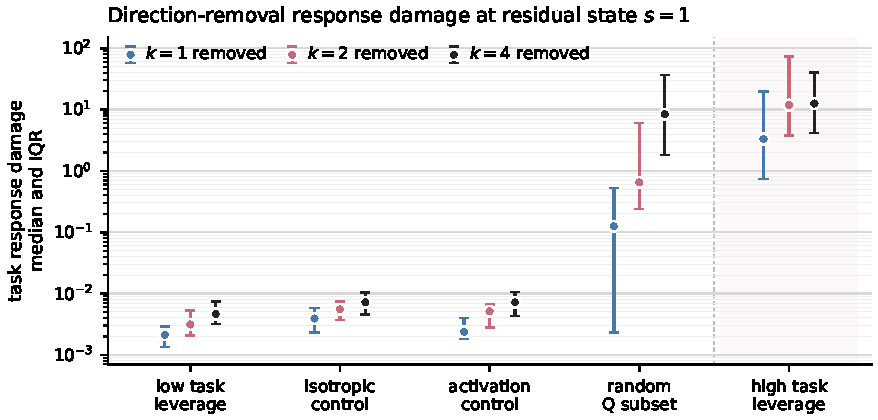
\includegraphics[width=0.78\linewidth]{../experiments/experiment_3_causal_surgery/results/experiment_3_key_surgery.pdf}
\caption{Experiment 3: selective causal effect of task-important activation directions. The plotted
metric is task finite-difference response damage. High task-leverage removals cause orders of
magnitude larger damage than matched low-task-leverage controls.}
\end{figure}

\begin{figure}[htbp]
\centering
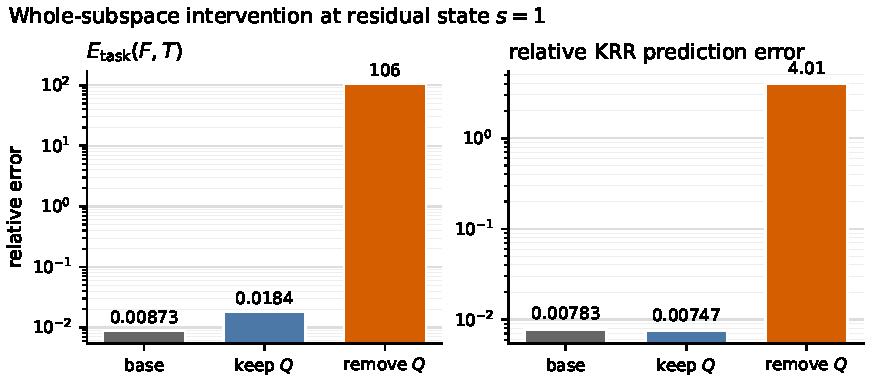
\includegraphics[width=0.82\linewidth]{../experiments/experiment_3_causal_surgery/results_complement_ablation/complement_ablation_bars.pdf}
\caption{Experiment 3: whole-subspace complement ablation at residual state \(s=1\). Keeping only
the \(Q\)-projection nearly preserves the task-local response; removing \(Q\) destroys it.}
\end{figure}

\FloatBarrier

Together, the selective removals and complement ablation support the causal-use claim in an
operational sense. The directions that the reduced KRR operator identifies as task-important are not
merely decodable; preserving them largely preserves the task-local response, and removing them
selectively destroys it.

\section{What Is Justified}

The experiments justify a bounded mechanistic claim:

\begin{quote}
For the tested checkpoint, geometries, perturbation scale, and task-label probe distribution, the
transformer's local label response is well approximated by a reduced KRR operator induced by a
compact context-side activation subspace. In successful settings, layerwise response spans contain
a prediction-risk-rank subspace whose induced reduced operator is close to exact KRR; in the
original linear setting, high-task-leverage directions from this subspace are causally important for
the transformer's response.
\end{quote}

They do not justify stronger claims. They do not show that the transformer globally equals ridge
regression. They do not show that derivative matching at one sampled label vector implies equality
on a neighborhood. They do not show that the transformer literally executes the explicit algorithm
\[
y\mapsto QQ^\top y\mapsto K_tQQ^\top y
\]
as its internal program. They also do not show that architecture alone guarantees the behavior.
The prediction-risk rank calculation supplies a requirement for context-side subspaces; it is not
an SGD theorem.

The clean final formulation is:

\begin{quote}
The trained transformer locally realizes the ridge-regression label-response operator on
task-distributed directions. In the tested regime, this behavior is explained by a compact
context-side activation subspace whose induced reduced ridge operator approximates exact KRR at the
prediction-risk rank. The layerwise diagnostic tracks when such a subspace becomes available; the
causal intervention then asks whether the model actually uses the selected directions.
\end{quote}

\section{Logical Chain}

The argument can be read as a sequence of commitments, each narrower than the previous one:

\begin{enumerate}[label=\arabic*.]
\item Freeze the episode geometry \(G=(X_{\mathrm{ctx}},X_{\mathrm{tgt}})\).
\item Under fixed \(G\), ridge regression becomes \(T=K_tA^{-1}\).
\item Treat the transformer as a label map \(F:\R^{n_{\mathrm{ctx}}}\to\R^{n_{\mathrm{tgt}}}\).
\item Estimate the local response \(D_\varepsilon F(y)[u]\).
\item Test behavior by checking \(E_\varepsilon(F,T)\) on task-label probes.
\item Compute the prediction-risk rank \(r_T\) from \(C_G=K_tA^{-1/2}\) and \(R_{\mathrm{KRR}}\).
\item Extract activation-derived context-side candidate spans \(C_\ell\).
\item Order each candidate span by KRR-targeted energy and form prefixes \(Q_{\ell,k}\).
\item Construct the KRR-constrained reduced operator \(T_Q=K_tQQ^\top\).
\item Test subspace sufficiency with \(\rho_G(T_Q)\).
\item Test model-subspace alignment with \(E_\varepsilon(F,T_Q)\).
\item In causal runs, remove high-leverage \(Q\)-directions and check whether task-local response is damaged.
\end{enumerate}

This is the full mechanism story: behavioral similarity, a KRR-structured activation certificate,
prediction-risk-rank sufficiency, layerwise emergence of the relevant subspace, and causal
specificity of high-leverage directions where the intervention has been validated.

\end{document}
